%=============================================================================
% Thesis Template in LaTex
%
% File:  f-01-01-a-R-S.tex -- Classical Approach R-S
% Author(s): Jürgen Hackl <hackl@ibi.baug.ethz.ch>
%            Clemens Kielhauser <kielhauser@ibi.baug.ethz.ch>
%
% Creation:  27 Jan 2014
% Time-stamp: <Tue 2013-08-13 20:14 juergen>
%
% Copyright (c) 2014 Infrastructure Management Group (IMG)
%               http://ibi.ethz.ch
%
% More information on LaTeX: http://www.latex-project.org/
%=============================================================================

% ******
% Figure
% ******

% Document name
% =============

% f-00-00-a-Example.txt

% f  ... Figure
% 00 ... Chapter
% 00 ... Number of the figure
% a  ... Subfigure
% Ex ... Name of the figure


% Libraries
% =========

\usetikzlibrary{shapes,arrows}
\usetikzlibrary{positioning}
\usetikzlibrary{shadows}
\usetikzlibrary{backgrounds}
% \usepackage{verbatim}
\usetikzlibrary{automata}
\usetikzlibrary{arrows}
\usetikzlibrary{calc}
\usetikzlibrary{patterns}



% Styles
% ======

% Line Width
% ----------

\tikzstyle{hugeLine}=[line width=1.7pt]
\tikzstyle{bigLine}=[line width=1.3pt]
\tikzstyle{normalLine}=[line width=1pt]
\tikzstyle{smallLine}=[line width=.7pt]
\tikzstyle{tinyLine}=[line width=.5pt]

% Line Types
% ----------

\tikzstyle{Axis}=[smallLine,-to]
\tikzstyle{Line}=[normalLine]
\tikzstyle{Solid}=[fill=black!10]
\tikzstyle{Arrow}=[>=latex,smallLine,->]
\tikzstyle{Dimension}=[tinyLine,|-|]


% TikZ figure
% ===========

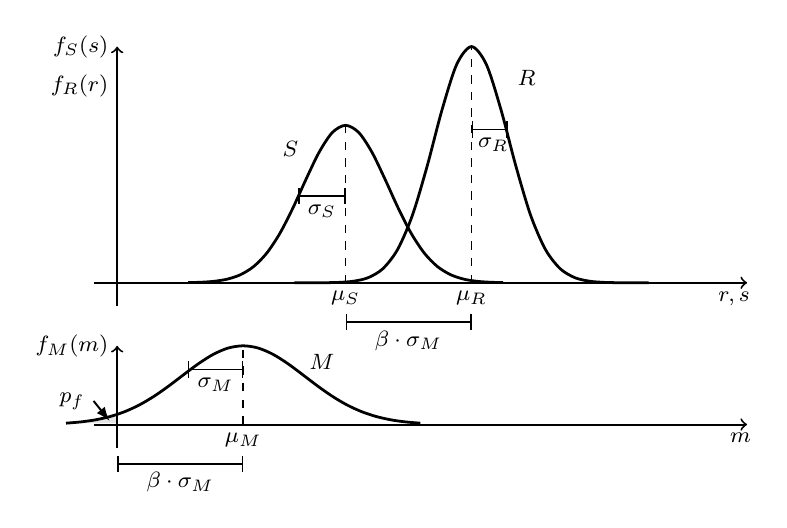
\begin{tikzpicture}


  % Grid
  % ----

  % \node [coordinate](ValA) at (0,0) {};
  % \node [coordinate](ValB) at (8,4) {};
  % \fill [fill=white](ValA) circle (.1pt);
  % \fill [fill=white](ValB) circle (.1pt);
  % \draw[help lines,step=1cm] (ValA) grid (ValB);

  \footnotesize

  % Distribution R
  \begin{scope}[xshift=4.5cm,yshift=0cm]
    \draw[tinyLine,dashed](0,0)--++(0,3) node [below,pos=0]{$\mu_R$};
    \draw[Dimension](0,1.95)--++(.46,0) node [below,pos=.6]{$\sigma_R$};
    \draw[Line,domain=-1.5:1.5,scale=1.5,smooth] plot (\x,{2*exp(-(\x)*(\x)*0.5/0.1)});
  \end{scope}

  \begin{scope}[xshift=2.9cm,yshift=0cm]
    \draw[tinyLine,dashed](0,0)--++(0,2) node [below,pos=0]{$\mu_S$};
    \draw[Dimension](0,1.1)--++(-.6,0) node [below,pos=.5]{$\sigma_S$};
  \draw[Line,domain=-2:2,scale=1,smooth] plot (\x,{2*exp(-(\x)*(\x)*0.5/0.3)});
  \end{scope}



  % \end{scope}

  % Axis
  \draw [Axis] (0,-.3)--(0,3) node [left, pos=1] {$f_S(s)$} node [left, pos=.85] {$f_R(r)$};
  \draw [Axis] (-.3,0)--(8,0) node [below, pos=.98] {$r,s$};

  % Comment
  \node (S) at (2.2,1.7){$S$};
  \node (R) at (5.2,2.6){$R$};
  \begin{scope}[xshift=0cm,yshift=-1.8cm]
  \begin{scope}[xshift=1.6cm,yshift=0cm]
    \fill[Solid,domain=-4.5:4.5,scale=.5,smooth] plot (\x,{2*exp(-(\x)*(\x)*0.5/2.5)});
    \fill[white](-1.6,0) rectangle (3.5,1);
    \draw[tinyLine,dashed](0,0)--++(0,1) node [below,pos=0]{$\mu_M$};
    \draw[Dimension](0,.7)--++(-.7,0) node [below,pos=.5]{$\sigma_M$};
    \draw[Line,domain=-4.5:4.5,scale=.5,smooth] plot (\x,{2*exp(-(\x)*(\x)*0.5/2.5)});
  \end{scope}

  % Dimension
  \draw[Dimension](0,-.5)--++(1.6,0) node [below,pos=.5]{$\beta\cdot \sigma_M$};

  % Arrow
  \draw [Arrow](-.3,.3)--(-.1,.05)node [left=0,pos=.0]{$p_f$};

  % Axis
  \draw [Axis] (0,-.3)--(0,1) node [left, pos=1] {$f_M(m)$};
  \draw [Axis] (-.3,0)--(8,0) node [below, pos=.99] {$m$};

  % Comment
  \node (M) at (2.6,.8){$M$};
  \end{scope}

  % Dimension
  \draw[Dimension](2.9,-.5)--(4.5,-.5) node [below,pos=.5]{$\beta\cdot \sigma_M$};

\end{tikzpicture}



% ===========================================================================
% EOF
%

%%% Local Variables:
%%% mode: latex
%%% TeX-master: "../main"
%%% End:
